%%%%%%%%%%%%%%%%%%%%%%%%%%%%%%%%%%%%%%%%%
% Wenneker Article
% LaTeX Template
% Version 2.0 (28/2/17)
%
% This template was downloaded from:
% http://www.LaTeXTemplates.com
%
% Authors:
% Vel (vel@LaTeXTemplates.com)
% Frits Wenneker
%
% License:
% CC BY-NC-SA 3.0 (http://creativecommons.org/licenses/by-nc-sa/3.0/)
%
%%%%%%%%%%%%%%%%%%%%%%%%%%%%%%%%%%%%%%%%%

%----------------------------------------------------------------------------------------
%	PACKAGES AND OTHER DOCUMENT CONFIGURATIONS
%----------------------------------------------------------------------------------------

\documentclass[12pt, a4paper, twocolumn]{article} % 10pt font size (11 and 12 also possible), A4 paper (letterpaper for US letter) and two column layout (remove for one column)
\usepackage{setspace}
\usepackage{multirow}
\usepackage{float}
\usepackage{hyperref}
\usepackage[USenglish,UKenglish,french,spanish,italian]{babel}
\usepackage{graphicx}
\graphicspath{ {./Immagini/} }

%%%%%%%%%%%%%%%%%%%%%%%%%%%%%%%%%%%%%%%%%
% Wenneker Article
% Structure Specification File
% Version 1.0 (28/2/17)
%
% This file originates from:
% http://www.LaTeXTemplates.com
%
% Authors:
% Frits Wenneker
% Vel (vel@LaTeXTemplates.com)
%
% License:
% CC BY-NC-SA 3.0 (http://creativecommons.org/licenses/by-nc-sa/3.0/)
%
%%%%%%%%%%%%%%%%%%%%%%%%%%%%%%%%%%%%%%%%%

%----------------------------------------------------------------------------------------
%	PACKAGES AND OTHER DOCUMENT CONFIGURATIONS
%----------------------------------------------------------------------------------------

% \usepackage[english]{babel} % English language hyphenation

\usepackage{microtype} % Better typography

\usepackage{amsmath,amsfonts,amsthm} % Math packages for equations

\usepackage[svgnames]{xcolor} % Enabling colors by their 'svgnames'

\usepackage[hang, small, labelfont=bf, up, textfont=it]{caption} % Custom captions under/above tables and figures

\usepackage{booktabs} % Horizontal rules in tables

\usepackage{lastpage} % Used to determine the number of pages in the document (for "Page X of Total")

\usepackage{graphicx} % Required for adding images

\usepackage{enumitem} % Required for customising lists
\setlist{noitemsep} % Remove spacing between bullet/numbered list elements

\usepackage{sectsty} % Enables custom section titles
\allsectionsfont{\usefont{OT1}{phv}{b}{n}} % Change the font of all section commands (Helvetica)

%----------------------------------------------------------------------------------------
%	MARGINS AND SPACING
%----------------------------------------------------------------------------------------

\usepackage{geometry} % Required for adjusting page dimensions

\geometry{
	top=1cm, % Top margin
	bottom=1.5cm, % Bottom margin
	left=2cm, % Left margin
	right=2cm, % Right margin
	includehead, % Include space for a header
	includefoot, % Include space for a footer
	%showframe, % Uncomment to show how the type block is set on the page
}

\setlength{\columnsep}{7mm} % Column separation width

%----------------------------------------------------------------------------------------
%	FONTS
%----------------------------------------------------------------------------------------

\usepackage[T1]{fontenc} % Output font encoding for international characters
\usepackage[utf8]{inputenc} % Required for inputting international characters

\usepackage{XCharter} % Use the XCharter font

%----------------------------------------------------------------------------------------
%	HEADERS AND FOOTERS
%----------------------------------------------------------------------------------------

\usepackage{fancyhdr} % Needed to define custom headers/footers
\pagestyle{fancy} % Enables the custom headers/footers

\renewcommand{\headrulewidth}{0.0pt} % No header rule
\renewcommand{\footrulewidth}{0.4pt} % Thin footer rule

\renewcommand{\sectionmark}[1]{\markboth{#1}{}} % Removes the section number from the header when \leftmark is used

%\nouppercase\leftmark % Add this to one of the lines below if you want a section title in the header/footer

% Headers
\lhead{} % Left header
\chead{\textit{\thetitle}} % Center header - currently printing the article title
\rhead{} % Right header

% Footers
\lfoot{} % Left footer
\cfoot{} % Center footer
\rfoot{\footnotesize Page \thepage\ of \pageref{LastPage}} % Right footer, "Page 1 of 2"

\fancypagestyle{firstpage}{ % Page style for the first page with the title
	\fancyhf{}
	\renewcommand{\footrulewidth}{0pt} % Suppress footer rule
}

%----------------------------------------------------------------------------------------
%	TITLE SECTION
%----------------------------------------------------------------------------------------

\newcommand{\authorstyle}[1]{{\large\usefont{OT1}{phv}{b}{n}\color{DarkRed}#1}} % Authors style (Helvetica)

\newcommand{\institution}[1]{{\footnotesize\usefont{OT1}{phv}{m}{sl}\color{Black}#1}} % Institutions style (Helvetica)

\usepackage{titling} % Allows custom title configuration

\newcommand{\HorRule}{\color{DarkGoldenrod}\rule{\linewidth}{1pt}} % Defines the gold horizontal rule around the title

\pretitle{
	\vspace{-30pt} % Move the entire title section up
	\HorRule\vspace{10pt} % Horizontal rule before the title
	\fontsize{25}{40}\usefont{OT1}{phv}{b}{n}\selectfont % Helvetica
	\color{DarkRed} % Text colour for the title and author(s)
}

\posttitle{\par\vskip 15pt} % Whitespace under the title

\preauthor{} % Anything that will appear before \author is printed

\postauthor{ % Anything that will appear after \author is printed
	\vspace{10pt} % Space before the rule
	\par\HorRule % Horizontal rule after the title
	\vspace{20pt} % Space after the title section
}

%----------------------------------------------------------------------------------------
%	ABSTRACT
%----------------------------------------------------------------------------------------

\usepackage{lettrine} % Package to accentuate the first letter of the text (lettrine)
\usepackage{fix-cm}	% Fixes the height of the lettrine

\newcommand{\initial}[1]{ % Defines the command and style for the lettrine
	\lettrine[lines=3,findent=4pt,nindent=0pt]{% Lettrine takes up 3 lines, the text to the right of it is indented 4pt and further indenting of lines 2+ is stopped
		\color{DarkGoldenrod}% Lettrine colour
		{#1}% The letter
	}{}%
}

\usepackage{xstring} % Required for string manipulation

\newcommand{\lettrineabstract}[1]{
	\StrLeft{#1}{1}[\firstletter] % Capture the first letter of the abstract for the lettrine
	\initial{\firstletter}\textbf{\StrGobbleLeft{#1}{1}} % Print the abstract with the first letter as a lettrine and the rest in bold
}

%----------------------------------------------------------------------------------------
%	BIBLIOGRAPHY
%----------------------------------------------------------------------------------------

\usepackage{biblatex} %Imports biblatex package
\addbibresource{sample.bib} %Import the bibliography file

\usepackage[autostyle=true]{csquotes} % Required to generate language-dependent quotes in the bibliography

\addto\captionsenglish{\renewcommand*\contentsname{Indice} } % Specifies the document structure and loads requires packages

%----------------------------------------------------------------------------------------
%	ARTICLE INFORMATION
%----------------------------------------------------------------------------------------

\title{Financial Market Analytics Project} % The article title

\author{
    Ruben Agazzi 844736\\
		Davide Abete 882299
}

%----------------------------------------------------------------------------------------

\begin{document}

\selectlanguage{USenglish}

% \maketitle % Print the title

\thispagestyle{firstpage} % Apply the page style for the first page (no headers and footers)

%----------------------------------------------------------------------------------------
%	ABSTRACT
%----------------------------------------------------------------------------------------
\twocolumn[
  \begin{@twocolumnfalse}
    \maketitle
    \begin{abstract}
			The project consist in the creation of portfolios, utilizing FTSE MIB index stocks, using different criteria in order to select the assets of the portfolios with a final analisys of the returns and risks of the portfolios
			\end{abstract}
  \end{@twocolumnfalse}]

\bigskip

\clearpage
% \lettrineabstract{x}
\bigskip
\tableofcontents

%----------------------------------------------------------------------------------------
%	ARTICLE CONTENTS
%----------------------------------------------------------------------------------------


	
	% Select between one and six entries from the list of approved keywords.
	% Don't make up new ones.
	
	%%%%%%%%%%%%%%%%%%%%%%%%%%%%%%%%%%%%%%%%%%%%%%%%%%
	
	%%%%%%%%%%%%%%%%% BODY OF PAPER %%%%%%%%%%%%%%%%%%
	\tableofcontents
	\section{Introduction} 
	In this project, the goal consists in creating different porfolios, using FTSE MIB index stocks, using different criteria in order to select the assests of the portfolios. Finally we make some analisys on the created portfolios, such as the returns and the level of risk of the portfolios, in order to see which one is the better performing.
	\section{Dataset}
	The dataset used consists in past data about the FTSE MIB index, in particular is composed of daily data about the past 5 years of every singular stock present in the FTSE MIB index, obtained using the yahoo finance API.
	\subsection{Dataset Columns}
	The dataset is composed by the following columns:
	\begin{itemize}
		\item Date: Date relative to the datas of the singular stock.
		\item Open: Opening price of the stock.
		\item High: Highest price reached by the stock in the current day.
		\item Low: Lowest price reached by the stock in the current day.
		\item Close: Closing price of the stock.
		\item Volume: Trading volume of the stocks.
		\item Adjusted Close: Closing price adjusted after accounting for any corporate actions.
		\item log ret: This column is calculated using the adjusted close prices, is the logarithm of the adjusted close price of the current day of the stock subtracted by the logarithm of the adjusted close price of the previous day.
	\end{itemize}
	
	\subsection{Data Exploration}
	The data did not present missing data so all the data is used inside the project.
	
	\section{Parameters}
	Afetr obtaining the data, we proceeded to obtain some parameters relative to the single stocks, in order to create the portfolios.
	\subsection{Rolling Regression}
	In order to obtain some of the parameters needed we proceeded to do a step of rolling regression on every single stock. The rolling regression was made using data about the past 180 days, and repeated for every week.
	The rolling regression is made using the Security Market Line(SML):
	\[
		r_i = \alpha_i +\beta_i(R_M)+e_i
	\]
	
	From the various rolling regressions we obtain the following parameters:
	\begin{itemize}
		\item Beta: is the beta coefficient obtained directly from the regression, this parameter indicates the Systematic Risk, in other words the risk that cannot be diversified away.
		\item Residual Variance($\sigma_{ei}$): Is the variance of the residuals of the regression.
		\item R-Squared: R-Squared statistic obtained from the rolling regression, indicates how well the regression can fit the data.
	\end{itemize}
	We decided to not use also the $\alpha$ coefficient because in most of the regressions it wasn't statistically significative.
	\subsection{Other parameters}
	The other parameters used to build the portfolios are:
	\begin{itemize}
		\item Log returns: weekly logarithmic returns of the single stock.
		\item Risk: weekly risk of the single stock, obtained by calculating the variance of the weekly returns of the stock.
	\end{itemize}
	
	\section{Portfolio Selection}
	In this phase we selected five different portfolios using different criteria. In general the portfolios are selected by ordering the weekly stock parameters in decrescent order, and selecting the top and bottom 10\% of the ordered stocks.
	The parameters used for the portfolio creation are:
	\begin{itemize}
		\item Beta Coefficient
		\item Stock variance
		\item Stock returns
		\item Residual variance
		\item R-Squared
	\end{itemize}
	\section{Portfolios Data}
	Using the mentioned parameters we obtained 5 different portfolios. For every portfolio we have obtained also the returns.
	\subsection{Portfolio returns}
	In order to obtain the portfolio returns we used the calculated weekly logarithmic returns, we made the inverse transformation in order to obtain the weekly return and multiplicated for the available investment.
	\[
	r_{t}	= r_{t-1}*e^{logret_{t}}
	\]
	\subsection{Beta Portfolio}
	This portfolio is obtained by taking the top and bottom 10\% of the stocks, odered by the beta parameter, and is rebalanced every week.\\
	The portfolio expected return,on the five years analized, is 107.89 euros, with an initial investment of 100 euros. The portfolio risk, calculated on the returns of a 100 euros investment, is equal to 4.73.
	\subsection{R-Squared Portfolio}
	This portfolio is obtained by taking the top and bottom 10\% of the stocks, odered by the R-Squared parameter, and is rebalanced every week.\\
	The portfolio expected return,on the five years analized, is 102.40 euros, with an initial investment of 100 euros. The portfolio risk, calculated on the returns of a 100 euros investment, is equal to 4.33.
	\subsection{Stock variance Portfolio}
	This portfolio is obtained by taking the top and bottom 10\% of the stocks, odered by their stock return variance, and is rebalanced every week.\\
	The portfolio expected return,on the five years analized, is 106.62 euros, with an initial investment of 100 euros. The portfolio risk, calculated on the returns of a 100 euros investment, is equal to 4.50.
	\subsection{Residual variance Portfolio}
	This portfolio is obtained by taking the top and bottom 10\% of the stocks, odered by their rolling regression residual variance, and is rebalanced every week.\\
	The portfolio expected return,on the five years analized, is 102.40 euros, with an initial investment of 100 euros. The portfolio risk, calculated on the returns of a 100 euros investment, is equal to 4.67.
	\subsection{Weekly returns Portfolio}
	This portfolio is obtained by taking the top 20\% of the stocks, odered by their weekly returns, and is rebalanced every week.\\
	This aproach is a strategy called Time Series Momentum Strategy, which consists in selecting the stocks of the portfolio by looking at past returns ant taking only the best performing stocks, in this case we used the previous week best performing stocks.
	The portfolio expected return,on the five years analized, is 108.99 euros, with an initial investment of 100 euros. The portfolio risk, calculated on the returns of a 100 euros investment, is equal to 4.76.
	\subsection{FTSE-MIB Portfolio}
	This portfolio is obtained by following the FTSE-MIB index.
	The portfolio expected return,on the five years analized, is 99.27 euros, with an initial investment of 100 euros. The portfolio risk, calculated on the returns of a 100 euros investment, is equal to 2.52.
	
	
	
	% La realizzazione di questo progetto ha avuto come obbiettivo quello di costruire diversi portafogli, ciascuno sulla base di specifici parametri come $R^2$, $\beta^2$ (rischio sistematico), $\sigma^2$ (rischio totale), al fine di effettuare un confronto in termini di rendimento medio atteso, volatilità e rapporto tra i due, di tutti i portafogli con il principale indice di benchmark dei mercati azionari italiani il FTSE MIB. Per fare ciò siamo partiti da una serie temporale giornaliera riguardante i prezzi di un insieme di stocks e abbiamo considerato come spazio temporale di investimento 5 anni, precisamente dal 2017-06-08 al 2022-06-08. Per ogni stock nell'arco temporale è stata eseguita una regressione dei log-returns ottenuti…(inserire calcolo) su un campione di 180 giorni, ottenendo $R^2$, $\alpha$ e $\beta$. Successivamente, abbiamo selezionato il primo e ultimo 10 per cento delle stocks ordinate in ordine decrescente sulla base ad esempio dell' $R^2$, al fine di costruire un portafoglio caratterizzato da assets di uguale peso, che è stato ribilanciato settimanalmente fino alla fine del campione.
	% \\Abbiamo calcolato i rendimenti settimanali di ciascuna stock, mediante la differenza tra il log-return corrente e quello della settimana precedente, al fine di calcolare i rendimenti settimanali dell'intero portafoglio come la media pesata dei rendimenti delle singole stock calcolate precedentemente. Inoltre, abbiamo ottenuto i rendimenti settimanali dell'indice FTSE MIB come la differenza tra il rendimento della settimana successiva e quello della settimana precedente. 
	% Dopo aver fatto queste operazioni, facendo partire il prezzo  da 100 e sommando o sottraendo a questo con cadenza settimanale il rendimento di ciascuna settimana, abbiamo potuto confrontare graficamente con un grafico delle serie storiche i rendimenti settimanali del portafoglio da noi costruito con i rendimenti settimanali dell'indice FTSE MIB, osservando come il rendimento del portafoglio sia prevalentemente maggiore di quello generato dall’indice.
	
	% Example table
	% \begin{table}[H]
	% 	\centering
	% 	\caption{Table containing the expected returns and risks of the created portfolios}
		
	% 	\begin{tabular}{ccccccc} % four columns, alignment for each
	% 		\hline
	% 		 / & Beta & R-Squared & Variance & Residual Variance & Return & FTSE-MIB \\
	% 		\hline
	% 		Expected Return & 102.07 & 99.12 & 102.48 &  99.12 &  99.12 & 99.27\\
	% 		Risk & 11.26 & 3.13 & 14.20 & 3.13 & 4.63 &  2.52\\
		
	% 		\hline
	% 	\end{tabular}
	% \end{table}
	\section{Results}
		Finally we made a table and a chart in order to compare all the portfolios.
	\begin{table}[H]
		\centering
		\caption{Table containing the expected returns and risks of the created portfolios, calculated with an initial investment of 100 euros}
		\begin{tabular}{cccc} % four columns, alignment for each
			\hline
			/ & A. Ret(\%) & A. Risk(\&) & Eff.(\%)\\
			\hline
			Beta & -2.86 & 34.07 & -9.1\\
			R-Squared & 1.2 & 31.23 & 3.5\\
			Variance & -3.39 & 32.47 & -10.44\\
			Res. Var. & 1.2& 33.7 & 3.56\\
			Return & -1.89 & 34.27 & -5.54\\
			FTSE MIB &  0.26 & 8.63 & 3.07\\
		
			\hline
		\end{tabular}
	\end{table}

		\begin{figure}[H]
			\caption{Line chart of portfolios returns}
			\begin{center}
				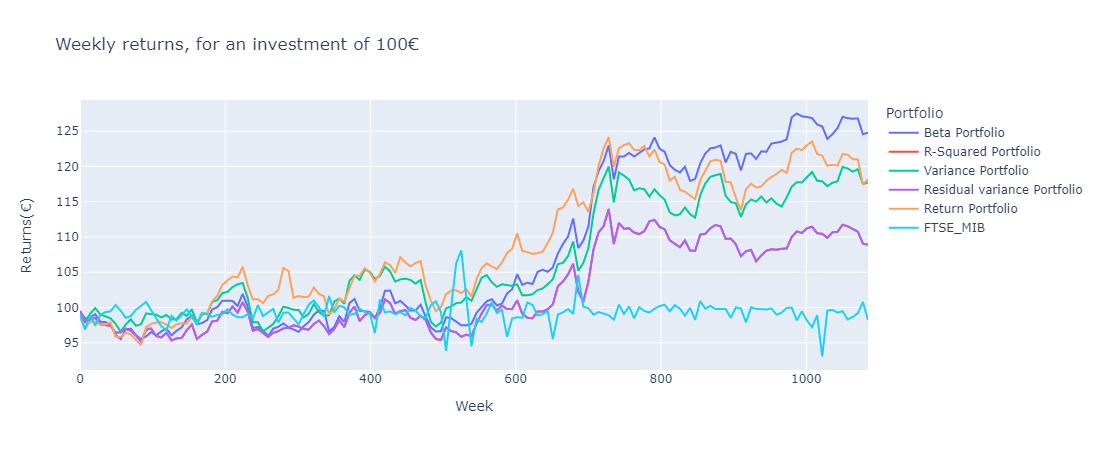
\includegraphics[width=75mm,scale=1]{port_ret_complete_small.png}
			\end{center}
		\end{figure}

	\section{Conclusions}
	As wee can see by the results the best performing portfolios are the ones built with Residuals variance and R-Squared as paramenters. Many portfolios have negative annual returns, probably this negative annual return is caused because the dataset contains daily data including the years 2020-2022; it is possible that theese bad results are caused by the covid 19 pandemic and the war in Ukraine.
\nocite{*} %aggiunge a bibliografia gli elementi non citati nel testo
\printbibliography[title={Bibliography}] %Prints bibliography

\end{document}
